\section{Gravitational Wave Example}
\label{sec: mc gw example}

\begin{table*}
\renewcommand{\arraystretch}{1.25}
\centering
\resizebox{\textwidth}{!}{
\begin{tabular}{lllll}
\hline\hline
Parameter & Description & True Population & VT Population & Strong Model Prior \\
\hline $\alpha$ & $m_1$ power-law index & $3.4$ & $3$ & 3.4 \\
$\beta_q$ & $q$ power-law index & $1.1$ & 1 & $1.1$ \\
$m_\mathrm{min}$ & minimum BH mass & $5M_\odot$ & $5M_\odot$ & $5M_\odot$ \\
$m_\mathrm{max}$ & maximum BH mass & $87M_\odot$ & $100M_\odot$ & $87M_\odot$\\
$\lambda_\mathrm{peak}$ & fraction of BBHs in Gaussian component & $0.04$ & $0.05$ & $0.04$ \\
$\mu_m$ & $m_1$ Gaussian component mean & $34M_\odot$ & $35 M_\odot$ & $34M_\odot$ \\
$\sigma_m$ & $m_1$ Gaussian component standard deviation  & $3.6M_\odot$ & $5M_\odot$ & $3.6M_\odot$  \\
$\delta_m$ & low-mass smoothing parameter & $4.8M_\odot$ & $4M_\odot$ & $4.8M_\odot$ \\
\hline
$\kappa$ & $z$ power-law index & $2.73$ & 2 & $2.73$ \\ 
\hline
$\alpha_\chi$ & spin magnitude $\alpha$ in Beta distribution & 1.67 & 1 & --- \\
$\beta_\chi$ & spin magnitude $\beta$ in Beta distribution & 4.43 & 1 & --- \\ 
$\mu_\chi$ & implied mean of spin magnitude Beta distribution & $0.274$ & $0.5$ & $U(0, 1)$ \\
$\sigma^2_\chi$ & implied variance of spin magnitude Beta distribution & $0.028$ & $0.083$ & $U(0.005, 0.25)$\\ \hline
$f_{q=1}$ & fraction in cosine-tilt Gaussian at equal mass ratio & 1 & 0 & 1 \\
$n$ & index in mass ratio, cosine-tilt correlation & 2 & --- & 2 \\
$\mu_\tau$ & mean of cosine-tilt Gaussian & 1 & --- & 1 \\
$\sigma_\tau$ & width of cosine-tilt Gaussian & 1.15 & --- & 1.15 \\
\hline\hline
\end{tabular}}
\caption{Parameters for the simulated population. In the ``True Population'' column, we show the true numerical values from \citet{Vitale:2025lms}. The ``VT Population'' column shows the parameter values for the source population for estimating selection effects. The ``Strong Model Prior'' column shows the model priors in our strong model (Beta spin distribution). Wherever we list a numerical value for a prior, we use a delta function prior at the true population value.}
\label{tab:true_hyper}
\end{table*}

To show how this works in a realistic \ac{GW} case, we show example hierarchical inferences with synthetic \ac{GW} source populations. We implement the hierarchical likelihood using \texttt{gwpopulation} \citep{Talbot:2019okv, Talbot:2024yqw}, and sample the posterior estimator using the \texttt{Bilby} \citep{Ashton:2018jfp} implementation of \texttt{dynesty} \citep{Speagle_2020}.
As our \ac{GW} source population, we use the large catalog described in \citet{Vitale:2025lms}. For estimating the selection efficiency, we created a injection set with $\Ninj = 4\times 10^9$ total injections, using a network of the Hanford and Livingston \ac{GW} interferometers with sensitivity defined in \citet{O4_psds}. We used a slightly stricter detection threshold than that used in \citet{Vitale:2025lms}.\footnote{We defined the network matched filter SNR as the \textit{real} parts of the matched filter SNRs summed in quadrature, where \citet{Vitale:2025lms} used the magnitude. \citet{Vitale:2025lms} also used a Virgo interferometer in addition to Hanford and Livingston. Therefore, the network SNRs computed in \citet{Vitale:2025lms} are always larger than the SNRs we compute here, so it is safe to down-select: a detection for our catalog is always a detection in \citet{Vitale:2025lms}.} Therefore, we down-selected the 1599 detections described therein to 1066 detections in order to be consistent with our selection criteria. We consider a catalog of 200 observations and a catalog of 1000 observations, and we show the following.

\begin{enumerate}
    \item We show further examples of the uncertainty in a posterior estimator and the quantification with the error statistic. We show how the inferred \ac{GW} populations can be subject to large errors if adequate error statistics are not met.
    \item For simple, strong models with well-constrained hyperparameters, thresholding on estimator convergence may be unnecessary (such as a log-likelihood variance threshold). The analyst can instead show the error statistic $\hat{E}[\hat{p}] \lesssim 0.2$ bits to demonstrate a safe analysis. 
    \item For weaker models, such as nonparametric models, it is necessary to adopt some sort of threshold to ensure a reliable posterior estimator. Thresholding on the log-likelihood variance is the only way to \textit{guarantee} that an analysis is safe, but other heuristic thresholds (e.g. based on Monte Carlo effective samples sizes $\Neff$) may be adopted, so long as the error statistic is shown to be small.
\end{enumerate}

\begin{figure}[h!]
    \centering
    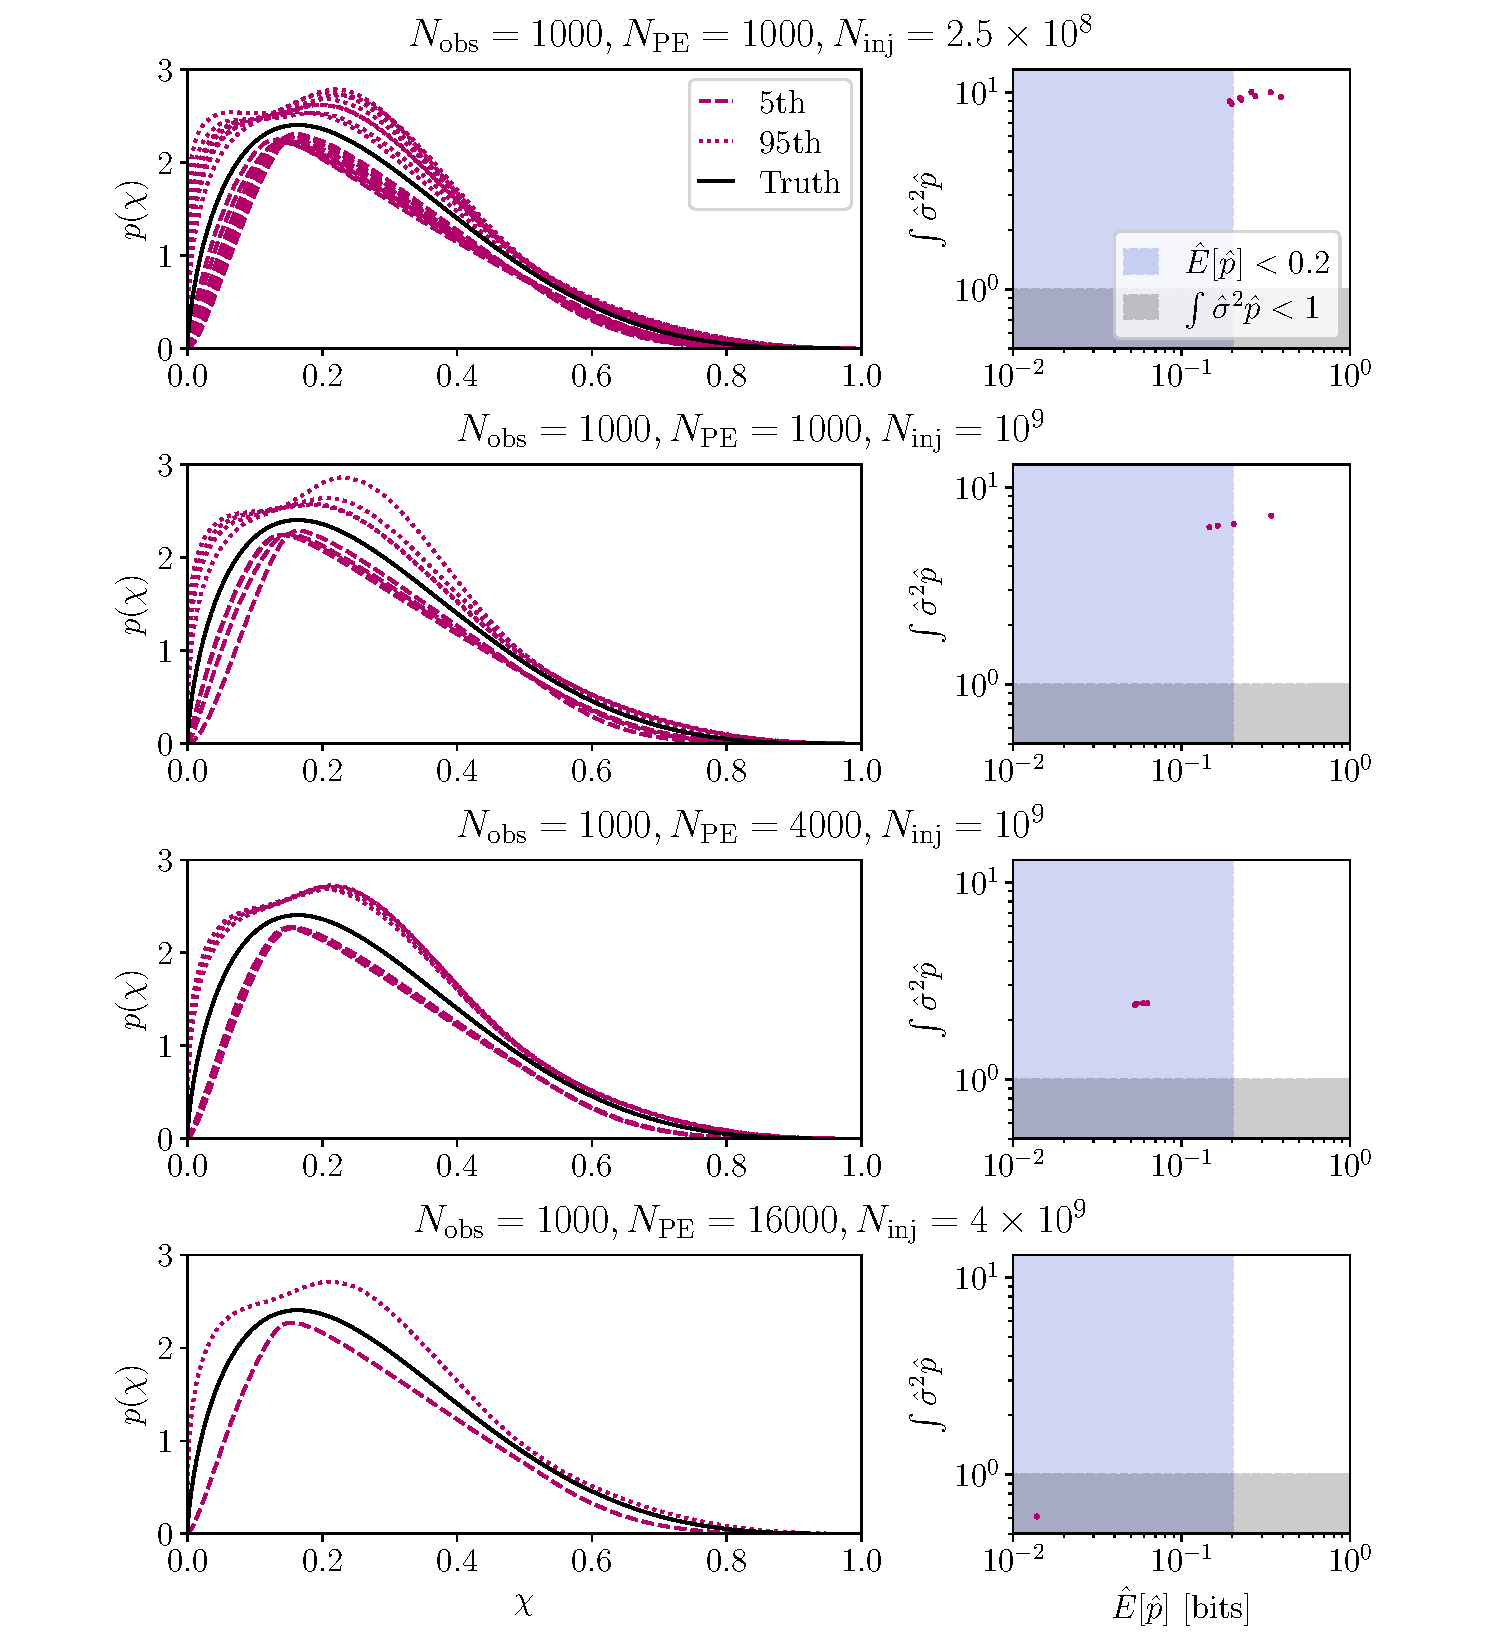
\includegraphics[width=0.78\linewidth]{plots/gw/spins/comparison_strong.pdf}
    \caption{The inferred spin distributions for different independent posterior estimators using a strong model. We have $\Nobs = 1000$ observations, and we vary the number of independent \ac{PE} samples $\NPE$ and the number of injections $\Ninj$ for estimating the selection efficiency. In the top row, we have eight independent posterior estimators with $\NPE = 1000$ and $\Ninj = 2.5\times 10^8$, the the second row we have four independent posterior estimators with $\NPE = 1000$ and $\Ninj = 10^9$, the third row has four independent posterior estimators with $\NPE = 4000$ and $\Ninj = 10^9$, and in the last row, we only have 1 posterior estimator with $\NPE = 16000$ and $\Ninj = 4\times 10^9$. In the left column we show the 90\% credible interval on the inferred spin distributions for each independent posterior estimator, where the dashed line is the $5^{\rm th}$ percentile and the dotted line is the $95^{\rm th}$ percentile. The black line shows the true spin distribution. In the right column we compare the error statistic $\hat{E}[\hat{p}]$ with the mean log-likelihood variance, showing that some inferences have log-likelihood variances greater than 1 but the error statistics are adequate and the inference is stable.}
    \label{fig:spins comparison strong}
\end{figure}

\begin{figure}[h!]
    \centering
    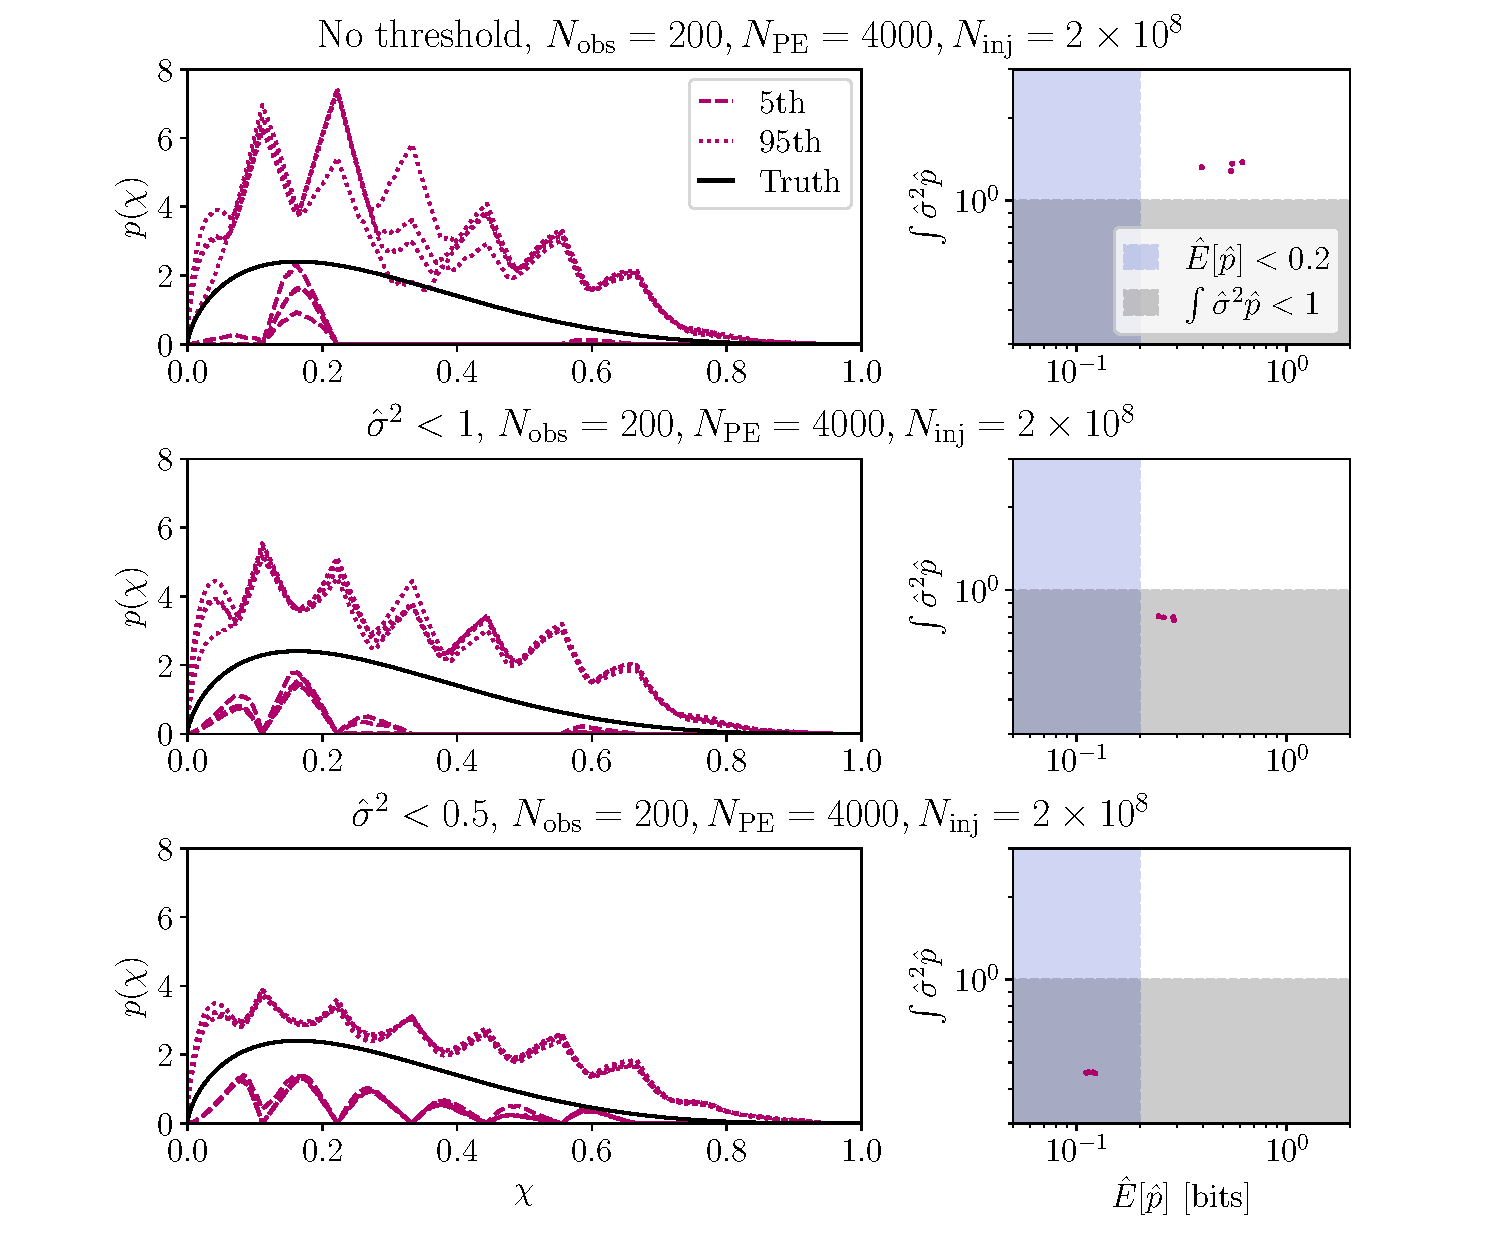
\includegraphics[width=0.78\linewidth]{plots/gw/spins/uniform_prior_comparison_weak_vs_varcut.pdf}
    \caption{Analogous to Fig.~\ref{fig:spins comparison strong} for a set of independent posterior estimators using a weak model, using $\Nobs = 200$ observations. Here we compare the impact of adopting different variance thresholds. In the top row, we use no threshold, and there is a significant amount of scatter between the independent posterior estimators (some even exclude the truth from the 90\% credible region). Adopting the fiducial variance threshold $\hat{\sigma}^2 < 1$ ensures significantly better behaved posterior estimators and an error statistic $\hat{E}[\hat{p}] \approx 0.25$ bits, which is acceptable although strains our recommendation $\hat{E}[\hat{p}] \lesssim 0.2$ bits. We show a further variance threshold for $\hat{\sigma}^2 < 0.5$ which places the error statistic well within the acceptable range, but at the cost of dramatically reducing the space of spin distributions explored.}
    \label{fig:spins comparison weak varcut}
\end{figure}

As discussed in Sec.~\ref{sec: mc gaussian example}, thresholding on the uncertainty can be more restrictive than is absolutely necessary. We use a strong spin model in Fig.~\ref{fig:spins comparison strong}, assuming a Beta distribution for the spins, where we infer the mean and variance of the Beta spin distribution as described in \citet{Wysocki:2018mpo} and \citet{KAGRA:2021duu}. In each row, we show the results of a number of inferences using unique realizations of $\NPE$ posterior samples for each observed event and unique realizations of $\Ninj$ draws for estimating the selection efficiency. For example, in the second row we show the results of 4 independent posterior estimators (we produced $4\times10^9$ samples from the VT population and so can down select to $4$ copies of $10^9$ unique sets for estimating the selection efficiency). In the left column, we show the $5^{\rm th}$ and $95^{\rm th}$ percentiles for the predicted spin distribution using the Beta spin model, as compared to the truth. We see some variation between different independent posterior estimators, and to estimate the degree of variation we compute the error statistic for each posterior estimator (the x-axis in the right column) compared to the average variance in the log-likelihood estimator (the y-axis in the right column). 


Notice in Fig.~\ref{fig:spins comparison strong} that the variance in the log-likelihood estimator can be as high as $\hat{\sigma}^2 \sim 10$, but the error statistic is in a tolerable range, $\hat{E}[\hat{p}] \lesssim 0.2$ bits. Furthermore, notice that the error statistic qualitatively tracks the degree of variation within the ensemble of posterior estimators (and verified quantitatively in Sections~\ref{sec: mc robustness measures} and \ref{sec: mc gaussian example}). For instance, with $\NPE = 4000$ and $\Ninj = 10^9$, the variance in the log-likelihood estimator is $\sim 2-3$. If the analyst was requiring that the log-likelihood variance was less than 1, this would require many more \ac{PE} samples and injections which can become computationally intractable. However, the error statistics are $\hat{E}[\hat{p}] \sim 0.05$ bits, well within a reliable range and indeed, the ensemble of 4 independent posterior estimators in the left column shows that the results are highly stable. 

Since the results with a strong model are stable with no convergence thresholds, they will also be reliable when using the effective sample size threshold. However, analysts should still be careful if they use an effective sample size threshold and check the error statistic is small in order to ensure the systematic uncertainty is acceptable.

\begin{figure}
    \centering
    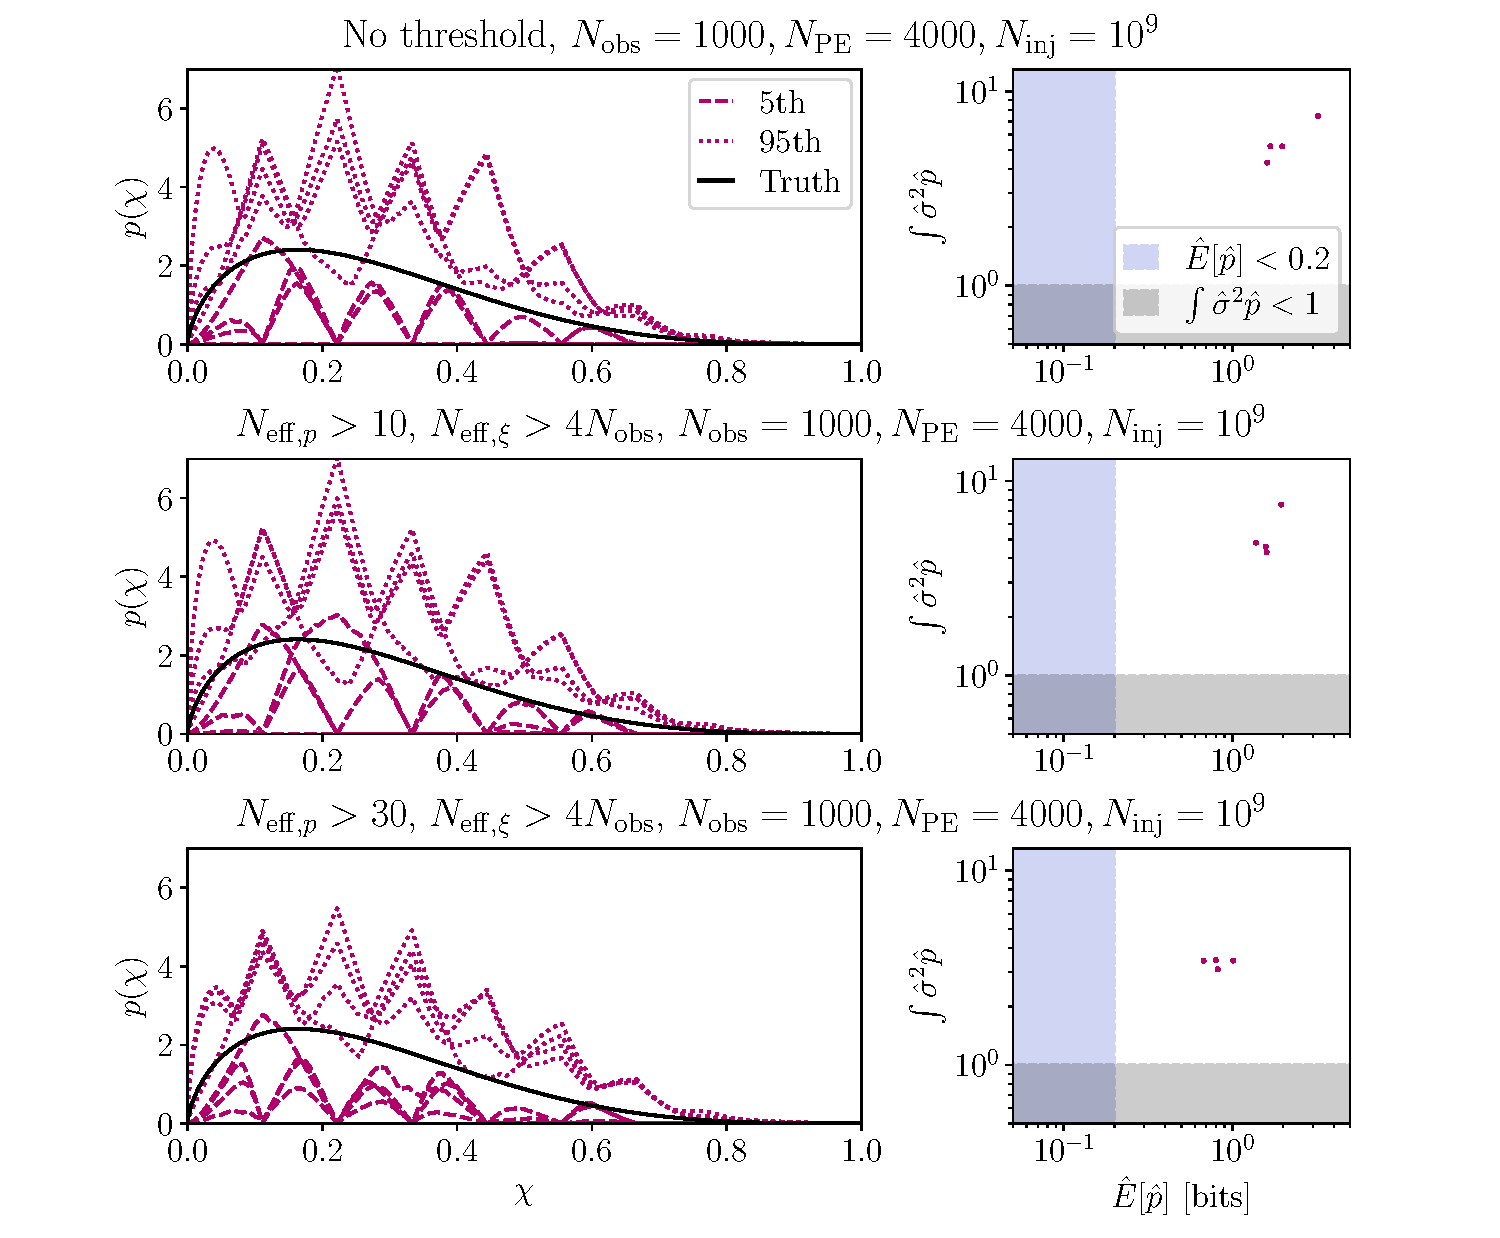
\includegraphics[width=0.78\linewidth]{plots/gw/spins/uniform_prior_comparison_weak.pdf}
    \caption{Analogous to Fig.~\ref{fig:spins comparison weak varcut} with $\Nobs = 1000$ detections. Here we compare the impact of adopting effective sample size thresholds. Note that none of the inferences shown here are reliable: the independent posterior estimators are quite different, reflected by the large error statistics computed in each inference. Note the log-likelihood variances are large in each of these inferences as well. These represent an example of the insufficiency of effective sample size thresholds \textit{on their own} to produce a reliable posterior estimator. In each of these, we also check that the effective sample size for the selection function estimator $N_{{\rm eff},\xi} \gtrsim 10^5 > 4\Nobs=4000$ to satisfy the threshold proposed in \citet{Farr:2019rap}.}
    \label{fig:spins comparison weak}
\end{figure}

We also show results using a weaker model (sometimes referred to as a data-driven or nonparametric model in the \ac{GW} community) for the spin distribution
\begin{equation}
    p(\chi|\{s_n\}) \propto p(\chi|\alpha_{\chi} = 1.67, \beta_{\chi} = 4.43)L(\chi| \exp[\{s_n\}])
    \label{eq: weak spin model}
\end{equation}
where $L(\chi|\exp[\{s_n\}])$ is a linear interpolation for $\chi$ between the nodes $(\chi_n, e^{s_n})$. In log space, this represents adding a linear interpolation scattering term to a base-Beta distribution (using the true population values), similar to the Power Law Spline models in \citet{Edelman:2021zkw, KAGRA:2021duu, Edelman:2022ydv, Godfrey:2023oxb}. We use 10 linear interpolation nodes and the x-axis positions of the nodes are separated linearly between 0 and 1. We use a uniform prior on $s_n \sim U(-10, 10)$ between $-10$ and $10$. Note if all $s_n=0$, then the spin population model reduces to the true spin distribution.

When using a weaker model as in Eq.~\ref{eq: weak spin model}, the resulting hyperposterior will be broader. The posterior estimator is well converged if, for each point in the support, the log-likelihood variance in that point is equally balanced by that point's average covariance with another point in the posterior. Over a larger hyperposterior support, we do not expect the covariance in the log-likelihood estimator surface to balance the variance. In such cases, the analyst may be forced to threshold on the uncertainty in the likelihood estimator, \textit{a posteriori} rejecting samples where some convergence statistic exceeds some threshold. Common thresholds considered in the literature are based on the effective sample size of individual Monte Carlo integrals \citep[e.g.][]{KAGRA:2021duu, Farr:2019rap} or on the total variance in the log-likelihood estimator \citep{Talbot:2023pex}. 

We showed in Section~\ref{sec: mc robustness measures} that a threshold on the variance of the log-likelihood estimator is \textit{guaranteed} to bound the overall error in the posterior estimator, and we suggested that thresholds on the effective sample size may not be sufficient. Here, we show two examples to demonstrate that (Fig.~\ref{fig:spins comparison weak varcut}) thresholding on the variance of the log-likelihood bounds the error in the posterior estimator and (Fig.~\ref{fig:spins comparison weak}) effective sample size thresholds are not always sufficient. 

In Fig.~\ref{fig:spins comparison weak varcut}, we compare the results between no threshold and a variance cut threshold, where we use $\Nobs = 200, \NPE = 4000, \Ninj = 10^8$. Without using any convergence threshold, there is a large amount of scatter between each posterior estimator and some exclude the true population from the 90\% credible region. Correspondingly, the error statistics are $\hat{E}[\hat{p}]\sim 0.6-0.8$ bits, too large to fall within the tolerable range. Once we turn on a variance threshold, the posterior estimators become much more reliable, and the error statistics drop towards a more acceptable $\hat{E}[\hat{p}] \sim 0.25$ bits, though they are still straining the recommended range $\hat{E}[\hat{p}] \lesssim0.2$ bits. However, the space of populations which can be explored is more limited. 
We also consider an even stricter threshold, where the variance in the log-likelihood is required to be less than $0.5$. The error statistic of these inferences are now well within the acceptable range $\hat{E}[\hat{p}] \sim 0.1$ bits, but at the cost of a severe reduction in the range of hyperparameters allowed by the variance threshold.

In Fig.~\ref{fig:spins comparison weak}, we show how effective sample size thresholds can sometimes be insufficient. We expect this to be particularly bad for weak models with a large number of observations, where the uncertainty in the likelihood is large and there may not be much covariance across the support of the posterior. 
We compare thresholds where $N_{{\rm eff}, p} > 10$, $N_{{\rm eff}, p} > 30$, and an example without any single-event Monte Carlo integral convergence threshold. In each example we additionally ensure that the effective sample size for the selection function estimator $N_{{\rm eff},\xi} > 4\Nobs$ to satisfy the threshold proposed in \citet{Farr:2019rap}. In practice, the effective sample size of the selection function estimator is $N_{{\rm eff},\xi} \gtrsim 10^5$, well above the suggested threshold and so it does not come into play. Notice the large scatter between independent posterior estimators (the 5th and 95th percentiles on the inferred spin distribution can be significantly different across independent sets of $\NPE$ and $\Ninj$ parameter estimation samples and injection set samples), and that some even exclude the truth.





